\documentclass{../tuda-beamer}


% Title information
\authors{Simon Hock}
\authors{Nhan Huynh}
\authors{Daniel Mangold}
\date{17. November 2021}

\begin{document}

  \maketitle

  \begin{frame}{Organisatorisches}
    \begin{itemize}
      \item 24.11.2021 Präsenzsprechstunde im Raum in Raum S103/\textbf{223}!
      \item Erinnerung: Themenvorschläge im Forum
      \item Zusätzliche Materialien wie die Präsentationen sind im Moodle Forum zu finden.
    \end{itemize}
  \end{frame}

  \begin{frame}{Vererbung}
    \begin{itemize}
      \item Grundlegendes Konzept der Objektorientierung
      \item Modellierung von Hierarchien in der realen Welt mit Hilfe von Klassen
      \item Basisklasse: Generalisierung
      \begin{itemize}
        \item Verallgemeinerung eines Objekts mit seinem Verhalten
      \end{itemize}
      \item Abgeleitete Klassen: Spezialisierung
      \begin{itemize}
        \item Eigene Ausprägungen und eigenes Verhalten
      \end{itemize}
    \end{itemize}
  \end{frame}

  \begin{frame}{Beispiel Typhierachie}
    \begin{figure}[h]
      \centering
      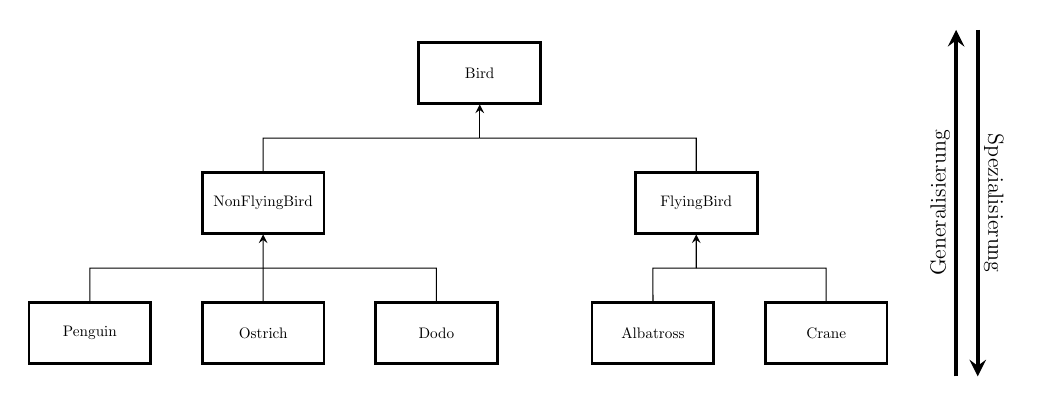
\begin{tikzpicture}[scale=.55, transform shape]
        \begin{scope}[
          every node/.style={
          draw,
          line width=1pt,
          minimum height=40pt,
          minimum width=80pt,
          transform shape,
          shape=rectangle,
          }
        ]
          \node (a) at (0, 0) {Bird};
          \node (b) at (-5, -3) {NonFlyingBird};
          \node (c) at (5, -3) {FlyingBird};
          \node (d) at (-9, -6) {Penguin};
          \node (e) at (-5, -6) {Ostrich};
          \node (g) at (-1, -6) {Dodo};
          \node (h) at (4, -6) {Albatross};
          \node (i) at (8, -6) {Crane};

          \draw[-stealth] (0, -1.5) -- (a);
          \draw (b.north) -- (-5, -1.5) -- (0, -1.5);
          \draw (c.north) -- (5, -1.5) -- (0, -1.5);

          \draw[-stealth] (e) -- (b);
          \draw (d.north) -- (-9, -4.5) -- (-5, -4.5);
          \draw (g.north) -- (-1, -4.5) -- (-5, -4.5);

          \draw[-stealth] (5, -4.5) -- (c);
          \draw (h.north) -- (4, -4.5) -- (5, -4.5);
          \draw (i.north) -- (8, -4.5) -- (5, -4.5);
        \end{scope}

        \draw[-stealth, ultra thick] (11, -7) -- node[rotate=90, above] {\Large Generalisierung}
        (11, 1);
        \draw[-stealth, ultra thick] (11.5, 1) -- node[rotate=270, above] {\Large Spezialisierung}
        (11.5, -7);
      \end{tikzpicture}
      \caption{Typhierarchie - Modellierung von Vögeln}
    \end{figure}
  \end{frame}

  \begin{frame}{Überschreiben von Methoden}
    \begin{itemize}
      \item Eigene Implementierung einer geerbten Methode
      \item Erlaubt das Funktionalitäten in der abgeleiteten Klasse zu verändern
      \item Gleichzeitig können aber die anderen Methoden der Oberklasse immer noch weiter verwendet
      werden.
      \item \inlinejava{@Override} Annotation (optional)
      \begin{itemize}
        \item Informiert den Compiler, dass das Element ein in einer Oberklasse deklariertes
        Element überschreiben soll.
      \end{itemize}
    \end{itemize}
  \end{frame}

  \begin{frame}[c]
    \lstinputlisting[style=Java, title=Erweiterung der Klasse Robot]{codes/FastRobot.java}
  \end{frame}

  \begin{frame}{Welche Implementierung wird ausgeführt?}
    \begin{itemize}
      \item Implementierung von \inlinejava{Robot}?
      \item Implementierung von \inlinejava{FastRobot}?
    \end{itemize}

    \vskip 3em

    \lstinputlisting[style=Java]{codes/Example_Override_Method.java}
  \end{frame}

  \begin{frame}{Überladen von Methoden}
    \begin{itemize}
      \item Methoden mit gleichem Namen können innerhalb einer Klasse definiert werden.
      \item Der Rückgabetyp kann beliebig sein, aber die Parameterlisten müssen verschieden sein.
    \end{itemize}

    \vskip 3em

    \begin{note}[title=Information:]
      Methoden werden nicht ausschließlich anhand ihres Namens identifiziert, sondern auch über die
      Typen, Anzahl und Reihenfolge ihrer Argumente (Parameter) - ihre Signatur.
    \end{note}
  \end{frame}

  \begin{frame}[c]{Überladen von Methoden - Beispiel}
    \lstinputlisting[style=Java]{codes/Point.java}
  \end{frame}

  \begin{frame}[c]
    \lstinputlisting[style=Java]{codes/Example_Overload_Method.java}
  \end{frame}

  \begin{frame}{Konstruktoren}
    \begin{itemize}
      \item Haben keinen Rückgabewert und der Name ist gleich dem Namen der Klasse.
      \item Konstruktoren werden nur einmal aufgerufen und zwar, wenn man ein neues Objekt erstellt.
      \item Konstruktoren werden nicht vererbt.
      \item Falls kein Konstruktor definiert wird, legt der Compiler einen leeren Konstruktor ohne
      Parameter an.
      \begin{itemize}
        \item Es gibt mindestens einen Konstruktor.
        \item Konstruktoren können überladen werden.
      \end{itemize}

      \lstinputlisting[style=Java]{codes/Constructor_Object.java}
    \end{itemize}
  \end{frame}

  \begin{frame}[c]
    \lstinputlisting[style=Java]{codes/Robot_Constructor.java}
  \end{frame}

  \begin{frame}{Schlüsselwort \inlinejava{this}}
    \begin{itemize}
      \item Referenzvariable, die auf das aktuelle Objekt verweist.
      \item Das Schlüsselwort \inlinejava{this} wird hauptsächlich in drei Situationen verwendet:
      \begin{itemize}
        \item Vermeidung von Mehrdeutigkeit von Variablenreferenzen
        \item Aktuelles Objekt als Argument, das an ein anderes Objekt übergeben wird
        \item Alternativer Konstruktoraufruf
      \end{itemize}
    \end{itemize}
  \end{frame}

  \begin{frame}{Vermeidung von Mehrdeutigkeit von Variablenreferenzen}
    \lstinputlisting[style=Java]{codes/Point.java}
  \end{frame}

  \begin{frame}{Aktuelles Objekt als Argument, das an ein anderes Objekt übergeben wird}
    \lstinputlisting[style=Java]{codes/Point_Argument_this.java}
  \end{frame}

  \begin{frame}[c]{Alternativer Konstruktoraufruf}
    \lstinputlisting[style=Java]{codes/Point_this_Constructor.java}
  \end{frame}

  \begin{frame}{Enums}
    \begin{itemize}
      \item Kurzform von Enumeration - Aufzählung
      \item Abgleitete Klassen von \href{https://docs.oracle.com/en/java/javase/11/docs/api/java
.base/java/lang/Enum.html}{java.lang.Enum}
      \item Bietet die Möglichkeit, vordefinierte Konstanten für Variablen festzulegen
      \item Nützliche Methode: \inlinejava{int ordinal()}: Gibt die Postion des Enums in der
      Enumdeklaration zurück.
    \end{itemize}
  \end{frame}

  \begin{frame}{Enum Direction - FOPBot}
    \lstinputlisting[style=Java]{codes/Direction.java}
  \end{frame}

  \begin{frame}[c]{Arbeitsphase}
    \begin{center}
      \textbf{\LARGE Selbstständiges Arbeiten}
    \end{center}
  \end{frame}
\end{document}
